\section{Abs\-Reverse$<$ Sets\-Type, Measure, Word, Cand\_\-Data\-Struct $>$ Class Template Reference}
\label{class_abs_reverse}\index{AbsReverse@{AbsReverse}}
Functor finding the negative border Bd- and/or the positive border Bd+ using the algorithm ABS doing a top dow exploration of the search space.  


{\tt \#include $<$Abs\-Reverse.hxx$>$}

Inheritance diagram for Abs\-Reverse$<$ Sets\-Type, Measure, Word, Cand\_\-Data\-Struct $>$::\begin{figure}[H]
\begin{center}
\leavevmode
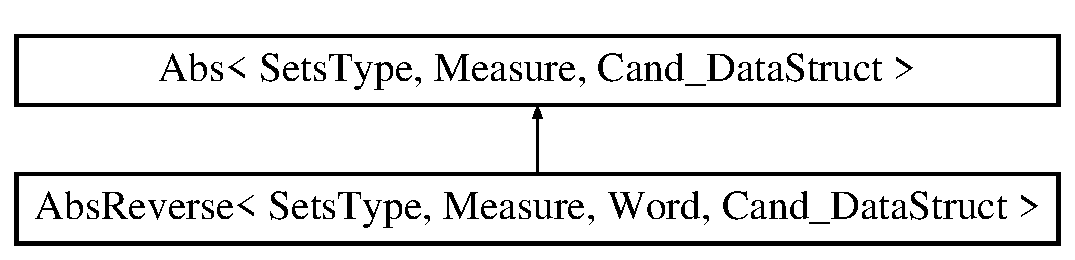
\includegraphics[height=2cm]{class_abs_reverse}
\end{center}
\end{figure}
\subsection*{Public Member Functions}
\begin{CompactItemize}
\item 
{\bf Abs\-Reverse} ()\label{class_abs_reverse_800fd75345935e7c59ee5058be8c4b1c}

\begin{CompactList}\small\item\em Constructor. \item\end{CompactList}\item 
{\bf $\sim$Abs\-Reverse} ()\label{class_abs_reverse_5a78f7a72b09b62b6e5326931890deef}

\begin{CompactList}\small\item\em Destructor. \item\end{CompactList}\item 
template$<$class Init\-Functor, class Predicate, class Stop\-Iteration, class Output\-Bd\-P, class Output\-Bd\-N, class f$>$ void {\bf operator()} (Init\-Functor \&init, {\bf Predicate} \&pred, Stop\-Iteration $\ast$stop\-Dualization, Output\-Bd\-P $\ast$out\-Bd\-P, Output\-Bd\-N $\ast$out\-Bd\-N, f \&word\-To\-Set)
\begin{CompactList}\small\item\em Functor operator that executes the algorithm. \item\end{CompactList}\item 
template$<$class Init\-Functor, class Predicate, class Stop\-Iteration, class Output\-Bd\-P, class Output\-Bd\-N$>$ void {\bf operator()} (Init\-Functor \&init, {\bf Predicate} \&pred, Stop\-Iteration $\ast$stop\-Dualization, Output\-Bd\-P $\ast$out\-Bd\-P, Output\-Bd\-N $\ast$out\-Bd\-N)
\begin{CompactList}\small\item\em Functor operator that executes the algorithm. \item\end{CompactList}\end{CompactItemize}


\subsection{Detailed Description}
\subsubsection*{template$<$class Sets\-Type = int, class Measure = Boolean, class Word = vector$<$ Sets\-Type $>$, class Cand\_\-Data\-Struct = PTree$<$Sets\-Type,Measure $>$$>$ class Abs\-Reverse$<$ Sets\-Type, Measure, Word, Cand\_\-Data\-Struct $>$}

Functor finding the negative border Bd- and/or the positive border Bd+ using the algorithm ABS doing a top dow exploration of the search space. 

The algorithme (\char`\"{}()\char`\"{} method)take in parameter: the initialisation functor, the predicate, the functor determining at which iteration the levelwise step is stop, the positive and/or negative borders (optional), the transformation function (optional).

The method execute\-Algorithm could be use to execute the algorithm. This method have another parameter to deal with \char`\"{}almost interesting elements\char`\"{} based on an error function passed i n parameter. These elements are considered as interesting during the iterations, and at the end they are used to do a top-down traversal of the search space to find the latests elements of Bd+.

The template parameter Sets\-Type represents the type of the elements of the set representation. The template parameter Measure is the type of the value eventually associated with the word of the language. The template parameter Word represents the type of the elements of the language. The template parameter Cand\_\-Data\-Struct is the data structure type used by the algorithms to manipulate the candidates generated. 



\subsection{Member Function Documentation}
\index{AbsReverse@{Abs\-Reverse}!operator()@{operator()}}
\index{operator()@{operator()}!AbsReverse@{Abs\-Reverse}}
\subsubsection{\setlength{\rightskip}{0pt plus 5cm}template$<$class Sets\-Type = int, class Measure = Boolean, class Word = vector$<$ Sets\-Type $>$, class Cand\_\-Data\-Struct = PTree$<$Sets\-Type,Measure $>$$>$ template$<$class Init\-Functor, class Predicate, class Stop\-Iteration, class Output\-Bd\-P, class Output\-Bd\-N$>$ void {\bf Abs\-Reverse}$<$ Sets\-Type, Measure, Word, Cand\_\-Data\-Struct $>$::operator() (Init\-Functor \& {\em init}, {\bf Predicate} \& {\em pred}, Stop\-Iteration $\ast$ {\em stop\-Dualization}, Output\-Bd\-P $\ast$ {\em out\-Bd\-P}, Output\-Bd\-N $\ast$ {\em out\-Bd\-N})\hspace{0.3cm}{\tt  [inline]}}\label{class_abs_reverse_783d932854ce93bd14518406996d8090}


Functor operator that executes the algorithm. 

\begin{Desc}
\item[Parameters:]
\begin{description}
\item[{\em init}]functor initializing the interesting items wrt predicate. \item[{\em pred}]the predicate \item[{\em stop\-Dualization}]functor determining when the apiori execution must stop \item[{\em bd\-P}]output the positive border in the given objet (must have a push\_\-back( container, measure ) method). \item[{\em bd\-N}]output the negative border in the given objet (must have a push\_\-back( container, measure ) method). \end{description}
\end{Desc}


Reimplemented from {\bf Abs$<$ Sets\-Type, Measure, Cand\_\-Data\-Struct $>$} {\rm (p.\,\pageref{class_abs_1cb8186e971cbb42b54d29bab5ba1e01})}.\index{AbsReverse@{Abs\-Reverse}!operator()@{operator()}}
\index{operator()@{operator()}!AbsReverse@{Abs\-Reverse}}
\subsubsection{\setlength{\rightskip}{0pt plus 5cm}template$<$class Sets\-Type = int, class Measure = Boolean, class Word = vector$<$ Sets\-Type $>$, class Cand\_\-Data\-Struct = PTree$<$Sets\-Type,Measure $>$$>$ template$<$class Init\-Functor, class Predicate, class Stop\-Iteration, class Output\-Bd\-P, class Output\-Bd\-N, class f$>$ void {\bf Abs\-Reverse}$<$ Sets\-Type, Measure, Word, Cand\_\-Data\-Struct $>$::operator() (Init\-Functor \& {\em init}, {\bf Predicate} \& {\em pred}, Stop\-Iteration $\ast$ {\em stop\-Dualization}, Output\-Bd\-P $\ast$ {\em out\-Bd\-P}, Output\-Bd\-N $\ast$ {\em out\-Bd\-N}, f \& {\em word\-To\-Set})\hspace{0.3cm}{\tt  [inline]}}\label{class_abs_reverse_d4e6aa7d0f2e50db5d5e75ab5801fd51}


Functor operator that executes the algorithm. 

\begin{Desc}
\item[Parameters:]
\begin{description}
\item[{\em init}]functor initializing the interesting items wrt predicate \item[{\em pred}]the predicate \item[{\em stop\-Dualization}]functor determining when the apiori execution must stop \item[{\em bd\-P}]output the positive border in the given objet (must have a push\_\-back( container, measure ) method). \item[{\em bd\-N}]output the negative border in the given objet (must have a push\_\-back( container, measure ) method). \item[{\em word\-Toset}]transformation function \end{description}
\end{Desc}


Reimplemented from {\bf Abs$<$ Sets\-Type, Measure, Cand\_\-Data\-Struct $>$} {\rm (p.\,\pageref{class_abs_991fe73b7db6f50b75e434631187ec9a})}.

The documentation for this class was generated from the following file:\begin{CompactItemize}
\item 
F:/i\-Zi/algorithms/Abs\-Reverse.hxx\end{CompactItemize}
